\section{Les différentes attaques}
Une fois en possession des diverses informations, il existe un
très grand nombre d'attaques différentes pour retrouver le message
clair ou la clé utilisée pendant le chiffrement. Voyons les
attaques les plus utilisées.

\subsection{L'analyse des fréquences\label{sec:AnalyseFrequences}}
Exposée pour la première fois par Al-Kindi au IX\ieme~ siècle,
l'analyse fréquentielle permet de déchiffrer des chiffrements
simples. Dans le cas d'une substitution, les
caractères sont représentés par autre chose, mais leurs fréquences
d'apparition ne changent pas~; on peut donc alors facilement
retrouver le message initial, connaissant les fréquences
normales d'apparition des caractères dans la langue du message.

L'analyse des fréquences ne se limite pas aux lettres
individuelles~; l'analyse des digrammes\footnote{Groupe de deux
lettres.} peut aussi être très
pratique.
\\

On peut, via cette méthode, trouver la langue dans laquelle le
message est écrit, car chaque langue possède une fréquence
d'apparition des lettres unique (voir la figure \ref{fig:Frequences}).

Bien évidemment, la fréquence d'apparition des lettres peut varier
au sein d'une même langue selon certains critères (par exemple un
message d'origine militaire risque de contenir beaucoup
d'abréviations). Une analyse des fréquences aura donc des résultats
plus probables sur des messages d'une certaine longueur.

\begin{figure}[h]
  \centering
    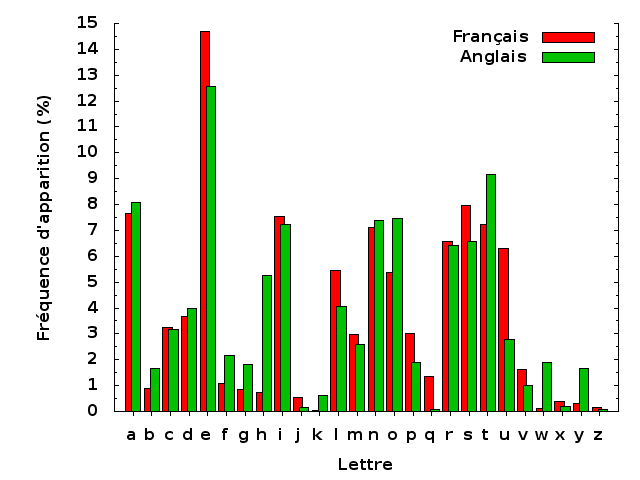
\includegraphics[width=0.9\textwidth]{plot/Frequences.png}
    \caption{fréquences d'apparition des lettres en français et en
anglais.}
  \label{fig:Frequences}
\end{figure}

Cette technique est par exemple expliquée dans la nouvelle
\emph{Le scarabée d'or} de Poe \cite{Poe}, qui s'était fortement 
intéressé à la cryptanalyse auparavant.


\subsection{L'indice de coïncidence}
Inventé en 1920 par William Friedman, l'indice de coïncidence
permet de découvrir à quel type de chiffrement on a affaire 
et dans le cas d'une
substitution polyalphabétique, il permet de trouver la taille de
la clé.

Cet indice représente en fait la probabilité que deux lettres
choisies au hasard dans un texte soient identiques. Comme pour
l'analyse des fréquences, cet indice varie selon la langue.
Ainsi, si l'indice de coïncidence d'un texte chiffré correspond à
celui d'une certaine langue, le texte est chiffré avec une
substitution monoalphabétique ou une transposition dans cette 
langue. Si, en revanche, l'indice ne correspond à rien, on a affaire 
à une substitution polyalphabétique.

Nous noterons l'indice de coïncidence propre au langage $I_l$, et
l'indice de coïncidence correspondant à un texte où les lettres
seraient placées uniformément $I_m$ (c'est en fait l'indice
minimal). 
\\

Calculons cet indice :
\begin{itemize}
  \item la probabilité que deux lettres tirées dans un texte est
égale à la probabilité de prendre deux A, plus la probabilité de
prendre deux B, \dots~ L'indice de coïncidence du texte est donc la
somme de ces probabilités :
  \begin{center}
    \[ Ic = p(\mbox{prendre deux A}) + p(\mbox{prendre deux B}) +
\dots + p(\mbox{prendre deux Z}) \]
  \end{center}
  \item Comme nous avons $C_{n}^2$ façons de prendre deux lettres
d'un texte de $n$ lettres, et $C_{n_A}^2$ façons de prendre deux A
dans ce même texte, s'il contient $n_A$ A, la probabilité de prendre 
deux A est
  \begin{center}
    \[ p(\mbox{prendre deux A}) = \dfrac{C_{n_A}^2}{C_{n}^2} =
\dfrac{\dfrac{n_A!}{2 (n_A - 2)!}}{\dfrac{n!}{2 (n - 2)!}} = 
\dfrac{n_A (n_A - 1)}{n (n - 1)} \]
  \end{center}
  \item L'indice de coïncidence devient alors, pour $n_i$
représentant la $i$\ieme~ lettre de l'alphabet :
  \begin{center}
    \[ Ic = \frac{n_1 (n_1 - 1)}{n (n - 1)} + \frac{n_2 (n_2 - 1)}{n
(n - 1)} + \dots + \frac{n_{26} (n_{26} - 1)}{n (n - 1)} = \sum_{i
= 1}^{26} \frac{n_i (n_i - 1)}{n (n - 1)} \] 
  \end{center}
\end{itemize}

Dans le cas d'une substitution polyalphabétique, comme le chiffre
de Vigenère, on pourrait diviser le message chiffré en plusieurs
parties, chacune de ces parties étant l'équivalent d'une
substitution simple, sur laquelle on pourrait procéder à une
analyse fréquentielle. Le nombre de parties étant égal à la
longueur de la clé, le plus important est alors de trouver la
longueur de la clé.

Considérons un message de $n$ caractères, chiffré avec une clé de
longueur $k$. Si nous écrivons ce message dans un tableau de $k$
colonnes, nous nous retrouverons avec un tableau de $\frac{n}{k}$
lignes, où chaque colonne correspondrait à une substitution
simple.

Si maintenant nous sélectionnons deux lettres dans ce tableau :
\begin{enumerate}
  \item soit elles se trouvent dans deux colonnes différentes, 
nous avons
alors $C_k^2 ~ (\frac{n}{k})^2$ façons de les choisir. Le nombre
de paires de lettres identiques au sein de deux colonnes distinctes
est alors
\[ I_m ~ C_k^2 ~ \left(\dfrac{n}{k}\right)^2 = 
I_m ~ \dfrac{k (k - 1)}{2} ~
\left(\dfrac{n}{k}\right)^2 = I_m ~ \dfrac{n^2 ~ (k-1)}{2k} \]
  \item soit elles se trouvent dans la même colonne, nous avons
alors $C_{\frac{n}{k}}^2 ~ k $ façons de les choisir. Le nombre de
paires de lettres % TODO: ortho ? singulier ou pluriel ?
identiques au sein d'une même colonne est
\[ I_l C_{\frac{n}{k}}^2 ~ k = I_l
\dfrac{n ~ (n-k)}{2k} \]
\end{enumerate}

On peut donc retrouver la valeur de l'indice de coïncidence du
texte :
\[Ic = \dfrac{I_m ~ \dfrac{n^2 ~ (k-1)}{2k} +
I_l \dfrac{n ~ (n-k)}{2k}}{C_n^2} =
\dfrac{I_m ~ n (k-1) + I_l (n-k)}{k ~
(n+1)} \]

De cette équation, on peut isoler $k$ :
\[k = \dfrac{n (I_l - I_m)}{n (Ic - I_m) + (I_l - Ic)} \]
Cette formule nous permet donc d'avoir une valeur assez proche de
la longueur de la clé.
\\

Nous pouvons assez simplement calculer $I_m$, l'indice d'un texte
contenant des lettres aléatoirement placées. Considérons un très
long texte de $n$ lettres, contenant toutes les lettres de
l'alphabet autant de fois les unes que les autres.
 Il est alors évident que le nombre de A
sera égal au nombre de B, au nombre de C, \dots~
Donc, $n_i$ (le nombre d'apparition de la $i$\ieme~ lettre de
l'alphabet dans le texte) vaudra $\dfrac{n}{26}$.
Comme $n$ est très grand, on considère que $n (n-1) = n^2$, et de
même pour $n_i$ : $\dfrac{n}{26} \left(\dfrac{n}{26} - 1\right) =
\left(\dfrac{n}{26}\right)^2$.
Calculons alors cet indice de coïncidence :

\[I_m = \dfrac{1}{n^2} \sum_{i = 1}^{26} \left(\dfrac{n}{26}\right)^2 =
\dfrac{1}{n^2} ~26~ \dfrac{n^2}{26^2} = \dfrac{1}{26} \approx
0,384\] 

\subsection{L'attaque par mot probable\label{sec:MotProbable}}
Quand on a la connaissance d'un mot qui pourrait être dans le
message chiffré, on a recours à cette attaque. On connaît alors le
mot en clair et en chiffré, on peut alors trouver des informations
pratiques sur la clé, ou bien un bout ou l'entièreté de la clé.

Dans l'annexe \ref{Apx:FBI}, nous verrons une simple mise en pratique
de cette méthode, couplée avec l'analyse des fréquences.

\subsection{L'attaque par force brute}
L'attaque par force brute est une attaque qui théoriquement
fonctionne à tous les coups. Elle consiste à essayer toutes les
clés possibles, une à une, jusqu'à ce qu'on retrouve
la clé utilisée pour le chiffrement.

Bien évidemment, à cause des restrictions matérielles, cette
technique prend énormément de temps pour trouver une solution. Ce
temps dépend de l'algorithme de chiffrement utilisé ainsi que de
la longueur de la clé. On comprend alors l'intérêt de choisir des
clés d'une certaine taille, afin de pouvoir résister à une attaque
par force brute (et cela ralentira aussi d'autres types
d'attaque).
\\

Il faut bien distinguer la longueur de la clé entre les
algorithmes de chiffrement symétriques et asymétriques, par
exemple, une clé de 1024 bits pour RSA (algorithme à clé
publique) correspond à une clé de 80 bits dans les algorithmes de
chiffrement symétriques. 

Dans le cas des chiffrements symétriques, pour une clé de $n$
bits, il existe alors $2^n$ clés possibles, c'est donc autant
d'opérations qu'il faudra effectuer afin de trouver la bonne clé. 
\\

On considère un algorithme de chiffrement cassé lorsque le nombre
d'opérations à effectuer pour casser un message est plus
petit que le nombre d'opérations qu'effectuerait une attaque par
force brute. Ainsi, dans le cas de la méthode de chiffrement
Triple DES, avec une clé de longueur de $2^{128}$ bits, une
attaque permet de casser un code en $2^{112}$ opérations (on dit
alors qu'il a 112 bits de sécurité). Ce nombre
reste très grand, mais l'algorithme est considéré comme cassé.
\\

Afin de pallier les limites matérielles, il existe diverses
méthodes permettant d'avoir accès à une puissance de
calcul considérable :
\begin{itemize}
  %\renewcommand{\makelabel}[1]{\sffamily\textbf{#1}}
  \item\sffamily{\textbf{le calcul distribué}} qui consiste, comme son nom
l'indique,
à distribuer le calcul sur différentes machines, qui effectueront
les opérations en tâche de fond. C'est utilisé par exemple dans
les nombreux projets nommés «~@home~» comme «~Folding@Home
»\footnote{Voir \url{http://folding.stanford.edu} pour plus
d'informations sur ce projet.},
organisé par l'université de Stanford et qui consiste à étudier
le repliement des protéines en fonction de divers facteurs, dans
le but de fabriquer de nouveaux médicaments~;
  \item\sffamily{\textbf{les fermes de calcul (ou clustering)}}, qui, comme le
calcul distribué, permettent de rassembler les puissances de
calculs de plusieurs machines excepté le fait que dans ce cas ci, cette
puissance de calcul sera uniquement utilisée pour la tâche
désirée~;
  \item\sffamily{\textbf{les machines spécialisées}}, comme c'est le cas de
\emph{Deep Crack}, une machine mise au point en 1998, qui déchiffra
un message en 56 heures lors du DES Challenge.\\
\end{itemize}

On peut aussi citer une méthode utilisée par certains logiciels pour
cracker les sommes MD5, qui consiste à utiliser la
puissance de calcul du processeur graphique (GPU) en plus de celle
du processeur (CPU). Ce genre de logiciel peut essayer dans les
meilleurs cas plus de
$2^{28}$ empreintes MD5 par seconde sur un ordinateur 
personnel et permet alors de retrouver le message clair en
moins d'une minute dans le cas d'un mot de passe simple\footnote{Test disponible à l'adresse
\url{http://fz-corp.net/repository/MD5-GPU.html}}.

\subsection{L'attaque par dictionnaire}
Cette attaque est souvent utilisée en parallèle avec l'attaque par
force brute, et consiste à essayer de déchiffrer un mot de passe
en essayant tous les mots d'une liste contenant des mots souvent
utilisés en tant que mot de passe.

Les logiciels procédant à ce type d'attaques (comme \emph{John the
Ripper}\footnote{Disponible sur
\url{http://www.openwall.com/john/}}) utilisent des «~règles~» à
partir de la liste de mots. Ces règles permettent d'essayer
plusieurs combinaisons utilisant le mot, ainsi, pour le mot
\texttt{password}, grâce aux règles, on pourra tester les mots
\texttt{password15}, \texttt{pAsSworD}, \texttt{p4ssw0rd}, \dots

Ce genre d'attaque (ainsi que l'attaque par force brute)
est grandement efficace contre des mots de passe. C'est
pour cela que l'on conseille de compliquer les mots de passe via
diverses méthodes, la plus efficace étant d'en générer un
aléatoirement via les nombreux sites internet nous offrant cette
possibilité\footnote{Comme
\url{http://www.eurnet.fr/passwd/passwd.html} qui informe aussi
du temps que tiendrait le mot de passe face à une attaque de type
% TODO: trouver un site libre
force brute ou par dictionnaire.} ou via une commande de ce genre sous les systèmes
de type Unix :
\lstset{language=bash}
\begin{lstlisting}
% < /dev/urandom tr -dc _A-Z-a-z-0-9 | head -c8 
\end{lstlisting}

\subsection{Le paradoxe des anniversaires}
Dans le cas d'une fonction de hachage, il y aura toujours des
collisions entre les sommes de contrôles de deux données
différentes, du fait que la taille du haché est définie, alors que
la taille des données peut être aussi longue qu'on le veut.
Dans le cas du MD5, la taille du haché est de 128 bits,
c'est-à-dire que l'on a $2^{128}$ hachés possibles.

Il peut être alors intéressant pour une personne malveillante de
trouver deux messages différents ayant la même somme de contrôle,
afin de remplacer un message par un autre, tout en laissant le
destinataire croire que le message est original et non modifié. Pour ce
faire, l'attaquant peut alors, via diverses modifications (ajouter
des espaces en fin de ligne, ajouter des lignes vides, …) essayer
de trouver une collision entre les sommes de contrôle des deux
messages. Mais combien de messages devra-t-il essayer avant d'en
trouver un qui correspond ?
\\

Illustrons cela par le problème des anniversaires : quelle est la
probabilité, en prenant une personne précise dans une pièce de $n$
personnes, qu'une autre personne de cette pièce ait son
anniversaire le même jour que cette personne ?

On peut reformuler cette phrase en «~Quelle est la probabilité, en
prenant une personne précise dans une pièce de $n$ personnes,
\emph{que personne d'autre dans cette pièce n'ait son anniversaire
le même jour que cette personne ?}~».

Pour chaque personne, la probabilité d'avoir son anniversaire un
jour différent de la personne choisie est de $\dfrac{364}{365}$.
La probabilité qu'une personne ait son anniversaire le même jour
que la personne choisie, parmi une pièce de $n$ personnes est de
\[ 1 - \left(\dfrac{364}{365}\right)^{n-1} \]

De cette équation, on peut trouver que pour avoir une probabilité
de $\dfrac{1}{2}$ : 
\[ n =
\dfrac{log\left(\dfrac{1}{2}\right)}{log\left(\dfrac{364}{365}\right)}
+ 1 \approx 264 \]

On peut donc dire que quand $n \geq 264$, cette probabilité est
supérieure à $\dfrac{1}{2}$. Pour généraliser, on dira que pour
trouver une personne ayant le même anniversaire qu'une autre
personne (précisée), il faudra regarder l'anniversaire d'environ
$365$ personnes.
\\

Regardons maintenant la probabilité de prendre deux personnes
ayant leur anniversaire le même jour dans une pièce de $n$
personnes. C'est donc le complémentaire de « Toutes les personnes
de la pièce ont leur anniversaire le même jour ».
La première personne peut avoir son anniversaire n'importe quel
jour, la seconde tous les jours, sauf celui où est née la première
personne, …

Cette probabilité vaut donc
\[1 - \dfrac{365}{365} ~ \dfrac{364}{365} ~ \dots ~ \dfrac{365 - n
+ 1}{365} \]

En cherchant $n$ pour que cette probabilité vaille 
$\dfrac{1}{2}$, on trouve $n \approx 23$. Comme approximation, nous
dirons que $n \approx \sqrt{365} \approx 19$
\\

Nous pouvons alors utiliser ceci pour trouver le nombre
de sommes de contrôles à tester avant de trouver une collision.
Si l'attaquant, à partir d'une somme de contrôle $x$,
déterminée par $x = h(M)$ ($h$ étant la fonction de hachage, et
$M$ le message initial), essaie de trouver $M'$ tel que $h(M') =
h(M)$, il lui faudra alors, pour $h$ produisant une sortie sur $n$
bits, $2^n$ messages avant de trouver une collision.

Si maintenant, l'attaquant applique des modifications aux deux
messages en même temps, il ne lui faudra plus qu'essayer
$\sqrt{2^n}$ sommes de contrôles, soit $2^{\frac{n}{2}}$.
Pour avoir une fonction de hachage résistante aux collisions, il
faut donc que $n$ soit assez grand pour que l'attaquant ne puisse
pas faire ces $2^{\frac{n}{2}}$ opérations nécessaires.

\subsection{Cryptanalyse différentielle}
Découverte à la fin des années 1980, la cryptanalyse
différentielle analyse comment les différences dans les messages
clairs influencent les différences dans les messages chiffrés.
L'étude de ces différences renseigne alors l'attaquant de certains
bits de la clé. Il
faut donc alors être dans une situation d'attaque à texte clair
choisi (l'attaque à texte clair connu est aussi possible, mais
nécessite un plus grand nombre de textes connus). 

Nous n'allons pas plus développer cette attaque, qui serait bien
trop longue à décrire en détail dans ce travail.

%\subsection{Cryptanalyse linéaire}
%Ce type d'attaque à été inventé par Mitsuru Matsui en 1992 pour
%attaquer le chiffre FEAL, et a été publiée en 1993  dans une
%attaque contre le chiffrement DES.

\subsection{Autres attaques}
Il existe encore d'autres types d'attaque non abordées ici. Le
secteur de la cryptanalyse est en perpétuelle évolution, chacun
peut trouver de nouvelles méthodes de crypt\-analyse avec beaucoup
de travail et de connaissances.

Les attaques présentées ici ne sont faisables que sur des
algorithmes de chiffrements symétriques, les systèmes de
chiffrements utilisant un lien entre la clé publique et la clé
privée, on essayera plutôt d'exploiter ce lien pour trouver la
clé privée. Dans le cas de RSA, il faut factoriser le nombre $e$,
afin de trouver ses deux diviseurs, $p$ et $q$, on pourra alors
retrouver facilement la clé privée $d$. La sécurité de cet
algorithme réside alors dans la difficulté de factoriser un nombre
qui est le produit de deux grands nombres premiers.

